% !TEX TS-program = pdflatex
% !TEX encoding = UTF-8 Unicode

%%%%%%%%%%%%%%%%%%%%%%%%%%%%%%%%%%%%%%%%%
% Structured General Purpose Assignment
% LaTeX Template
%
% This template has been downloaded from:
% http://www.latextemplates.com
%
% Original author:
% Ted Pavlic (http://www.tedpavlic.com)
%
% Note:
% The \lipsum[#] commands throughout this template generate dummy text
% to fill the template out. These commands should all be removed when 
% writing assignment content.
%
%%%%%%%%%%%%%%%%%%%%%%%%%%%%%%%%%%%%%%%%%

%----------------------------------------------------------------------------------------
%	PACKAGES AND OTHER DOCUMENT CONFIGURATIONS
%----------------------------------------------------------------------------------------

\documentclass[12pt]{article}
\usepackage[utf8]{inputenc} % set input encoding (not needed with XeLaTeX)

\usepackage{fancyhdr} % Required for custom headers
\usepackage{lastpage} % Required to determine the last page for the footer
\usepackage{extramarks} % Required for headers and footers
\usepackage{graphicx} % Required to insert images
\usepackage{caption}
\usepackage{float}
\usepackage{listings}
\usepackage{url}
\usepackage{subcaption}
\usepackage{amssymb}
\usepackage{textcomp}
\usepackage{color}
\usepackage{pdfpages}
\usepackage[hidelinks]{hyperref}
\usepackage{tikz}

\def\checkmark{\tikz\fill[scale=0.4](0,.35) -- (.25,0) -- (1,.7) -- (.25,.15) -- cycle;} 

\definecolor{lightgray}{rgb}{.9,.9,.9}
\definecolor{darkgray}{rgb}{.4,.4,.4}
\definecolor{purple}{rgb}{0.65, 0.12, 0.82}

\lstdefinelanguage{JavaScript}{
  keywords={typeof, new, true, false, catch, function, return, null, catch, switch, var, if, in, while, do, else, case, break},
  keywordstyle=\color{blue}\bfseries,
  ndkeywords={class, export, boolean, throw, implements, import, this},
  ndkeywordstyle=\color{darkgray}\bfseries,
  identifierstyle=\color{black},
  sensitive=false,
  comment=[l]{//},
  morecomment=[s]{/*}{*/},
  commentstyle=\color{purple}\ttfamily,
  stringstyle=\color{red}\ttfamily,
  morestring=[b]',
  morestring=[b]"
}

\lstset{
   language=JavaScript,
   backgroundcolor=\color{lightgray},
   extendedchars=true,
   basicstyle=\footnotesize\ttfamily,
   showstringspaces=false,
   showspaces=false,
   numbers=left,
   numberstyle=\footnotesize,
   numbersep=9pt,
   tabsize=2,
   breaklines=true,
   showtabs=false,
   captionpos=b
}

\hypersetup{colorlinks=false}

% Margins
\topmargin=-0.45in
\evensidemargin=0in
\oddsidemargin=0in
\textwidth=6.5in
\textheight=9.0in
\headsep=0.25in 


\linespread{1.1} % Line spacing

% Set up the header and footer
\pagestyle{fancy}
\lhead{\hmwkAuthorName} % Top left header
\chead{\hmwkClass\ \hmwkTitle} % Top center header
\rhead{\firstxmark} % Top right header
\lfoot{\lastxmark} % Bottom left footer
\cfoot{} % Bottom center footer
\rfoot{Page\ \thepage\ of\ \pageref{LastPage}} % Bottom right footer
\renewcommand\headrulewidth{0.4pt} % Size of the header rule
\renewcommand\footrulewidth{0.4pt} % Size of the footer rule

\setlength\parindent{0pt} % Removes all indentation from paragraphs

%----------------------------------------------------------------------------------------
%	DOCUMENT STRUCTURE COMMANDS
%	Skip this unless you know what you're doing
%----------------------------------------------------------------------------------------

% Header and footer for when a page split occurs within a problem environment
\newcommand{\enterProblemHeader}[1]{
\nobreak\extramarks{#1}{#1 continued on next page\ldots}\nobreak
\nobreak\extramarks{#1 (continued)}{#1 continued on next page\ldots}\nobreak
}

% Header and footer for when a page split occurs between problem environments
\newcommand{\exitProblemHeader}[1]{
\nobreak\extramarks{#1 (continued)}{#1 continued on next page\ldots}\nobreak
\nobreak\extramarks{#1}{}\nobreak
}

\setcounter{secnumdepth}{0} % Removes default section numbers
\newcounter{homeworkProblemCounter} % Creates a counter to keep track of the number of problems

\newcommand{\homeworkProblemName}{}
\newenvironment{homeworkProblem}[1][Problem \arabic{homeworkProblemCounter}]{ % Makes a new environment called homeworkProblem which takes 1 argument (custom name) but the default is "Problem #"
\stepcounter{homeworkProblemCounter} % Increase counter for number of problems
\renewcommand{\homeworkProblemName}{#1} % Assign \homeworkProblemName the name of the problem
\section{\homeworkProblemName} % Make a section in the document with the custom problem count
\enterProblemHeader{\homeworkProblemName} % Header and footer within the environment
}{
\exitProblemHeader{\homeworkProblemName} % Header and footer after the environment
}

\newcommand{\problemAnswer}[1]{ % Defines the problem answer command with the content as the only argument
\noindent\framebox[\columnwidth][c]{\begin{minipage}{0.98\columnwidth}#1\end{minipage}} % Makes the box around the problem answer and puts the content inside
}

\newcommand{\homeworkSectionName}{}
\newenvironment{homeworkSection}[1]{ % New environment for sections within homework problems, takes 1 argument - the name of the section
\renewcommand{\homeworkSectionName}{#1} % Assign \homeworkSectionName to the name of the section from the environment argument
\subsection{\homeworkSectionName} % Make a subsection with the custom name of the subsection
\enterProblemHeader{\homeworkProblemName\ [\homeworkSectionName]} % Header and footer within the environment
}{
\enterProblemHeader{\homeworkProblemName} % Header and footer after the environment
}
   
%----------------------------------------------------------------------------------------
%	NAME AND CLASS SECTION
%----------------------------------------------------------------------------------------

\newcommand{\hmwkTitle}{`MyAlcoholFreeWine.com'} % Assignment title
\newcommand{\hmwkDueDate}{Monday,\ December\ 7,\ 2015} % Due date
\newcommand{\hmwkClass}{SE31520} % Course/class
\newcommand{\hmwkAuthorName}{James Euesden - jee22} % Your name

%----------------------------------------------------------------------------------------
%	TITLE PAGE
%----------------------------------------------------------------------------------------

\title{
\vspace{2in}
\textmd{\textbf{\hmwkClass:\ \hmwkTitle}}\\
\normalsize\vspace{0.1in}\small{Due\ on\ \hmwkDueDate}\\
\vspace{3in}
}

\author{\textbf{\hmwkAuthorName}}
\date{} % Insert date here if you want it to appear below your name

%----------------------------------------------------------------------------------------

\setlength\parindent{24pt}

\begin{document}

\maketitle

%----------------------------------------------------------------------------------------
%	TABLE OF CONTENTS
%----------------------------------------------------------------------------------------

%\setcounter{tocdepth}{1} % Uncomment this line if you don't want subsections listed in the ToC

\newpage
\tableofcontents
\newpage

%----------------------------------------------------------------------------------------
%	INTRODUCTION
%----------------------------------------------------------------------------------------

% To have just one problem per page, simply put a \clearpage after each problem

\section{Introduction}

The assignment task\cite{assignment} was to implement a web site using Ruby on Rails, and a Web Service with RESTful resources. The web site, MyAlcoholFreeWines.com (MAF), was to call two instances of the Web Service as Wine Suppliers, get their list of Wines and then display to a Customer the cheapest wines available, and place an order for them if they wished. This report serves to document the design, testing and structure of my application, and as self evaluation of work carried out. All Wine images used for the application are credited to StockVault\cite{stockvault} from their Free Wine Stock Photos gallery.

%----------------------------------------------------------------------------------------
%	MAF ARCHITECTURE
%----------------------------------------------------------------------------------------

\section{MAF Architecture}
My experience with Ruby on Rails before the assignment was very limited, and I was unsure how to begine. I knew I would be using MVC, and that I would have HTTP requests coming through the browser to RESTful endpoints on my controllers. The controllers would then talk to the model classes they were associated with, and the view would display what the controller had for them.

To get a good starting point for my application, the preliminary design was based on the example provided in the `Agile Web Development with Rails'\cite{railsbook} book, and then heavily modified in order to suit the requirements of the assignment. This starting point allowed me to see the MVC structure and how to begin writing the application.

In order to fulfill the requirements, I needed a number of entities: Wines, Customers, CustomerDetails, Baskets and BasketItems. These all have their own controllers, views and models, where their data is stored in a local Sqlite3 database during development. I also implemented a controller for Sessions, which refers to when a Customer is on the website and has a `session', allowing them to be logged in and retain a Basket as they navigate through the site.

I also knew that I had to have some way of storing the Wines when I got results back from the Web Services. I considered keeping them in memory, which might be okay for a very small application, but would be completely un-scalable for an application that could be used by many people at once and with multiple massively stocked Wine Suppliers to call to. I chose to keep the Wines received in a Database, where I would store all Wines provided by each supplier, but only the cheapest of each Wine.

\begin{figure}[H]
        \centering
                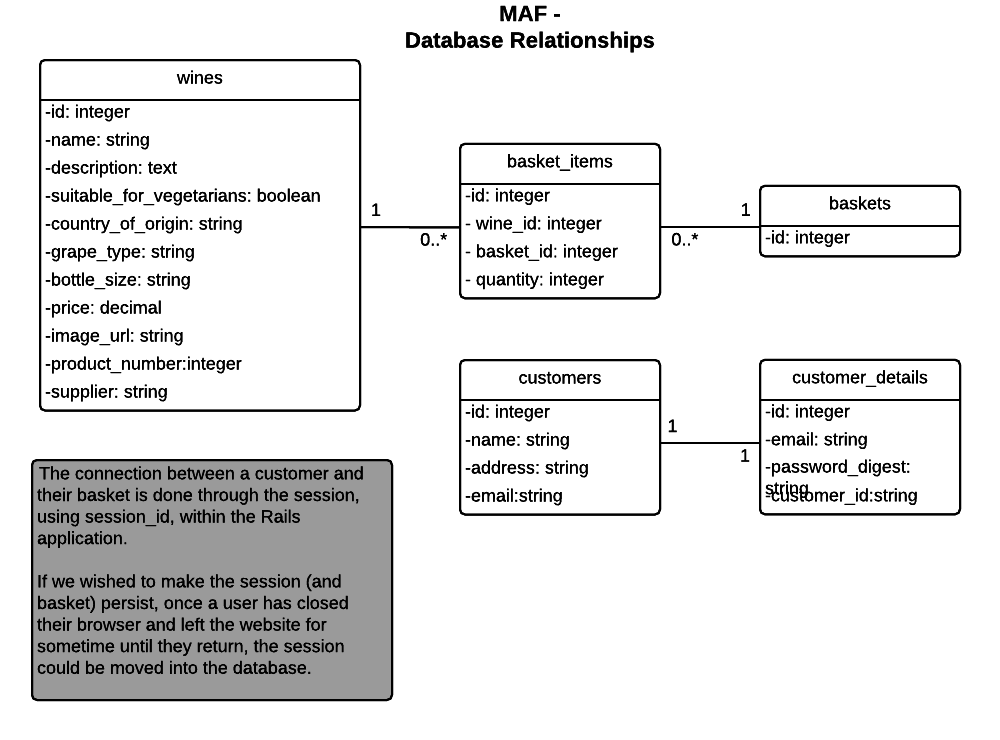
\includegraphics[width=1\textwidth]{assets/MAF_Database_relationships}
                \caption{The intended design of the database and relations between tables in the MAF application.}
                \label{fig: Intended MAF Database relationships.} 
\end{figure}

The representation of a BasketItem is for a many-to-many relationship, indicating that a Basket can have many Wines in it, and a Wine can be in many Baskets of different Customers. The connection between Customers and their Basket is done through the session parameter in Rails. I did consider having Session as an entity for storing in the database, and this would allow a user to retain their Basket and BasketItems for another time when they next login. However, I felt this was out of scope for the prototype.

I chose to keep the Supplier name as a field in the Wine entity, and the connections to these Suppliers is located in a configuration file. This could allow Suppliers to be updated through configuration once the site is deployed. However, I also know that there is the possibility of having a Table in the database for Web Suppliers which could contain their URIs, names and any additional needed information. Were I to re-implement this application, I may opt for that approach should more information about the Suppliers be required.

Based on what I expected to need, I made the target class design diagram that can be seen below. This shows the connections between the requests to MAF controllers and what the controllers connect to for their data and showing it.

\vspace*{\fill}
\begin{figure}[H]
        \centering
\noindent\makebox[\textwidth]{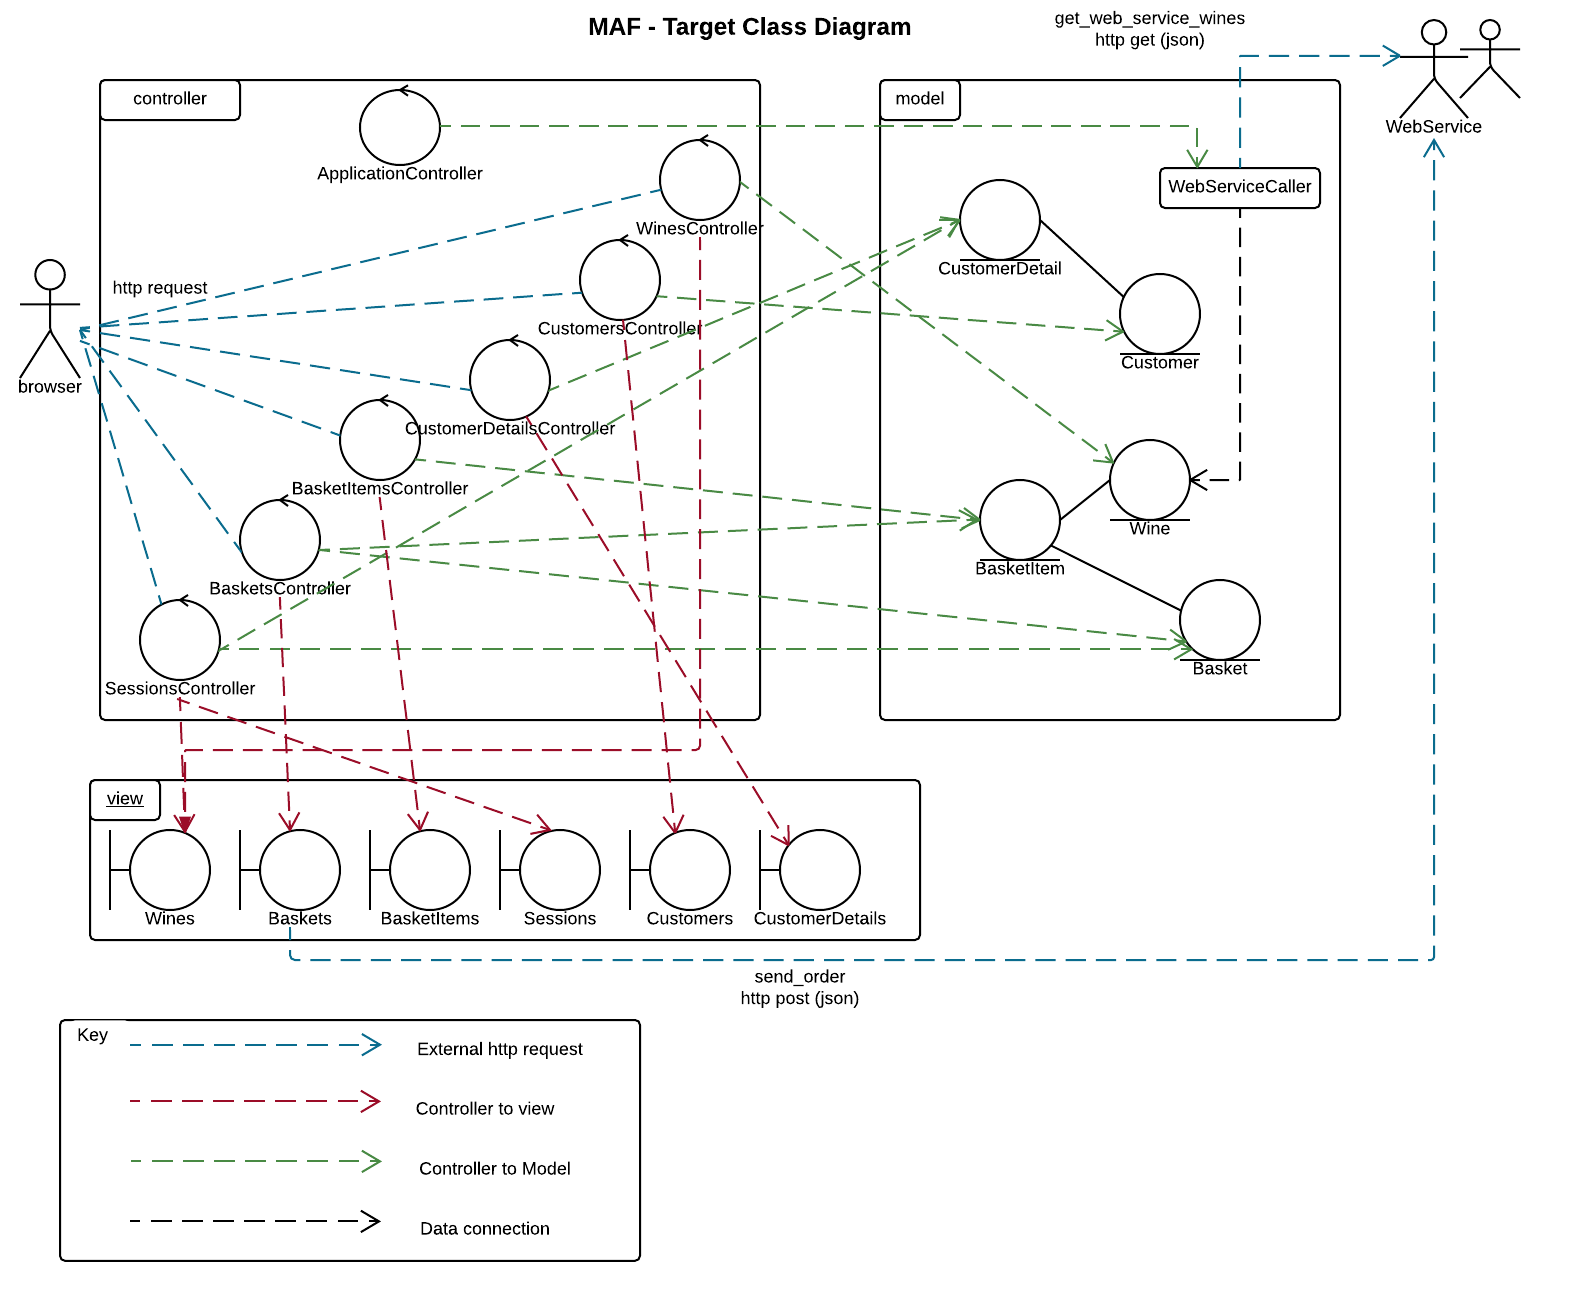
\includegraphics[width=1.2\textwidth]{assets/MAF_Target_Class_Design}}%
                %%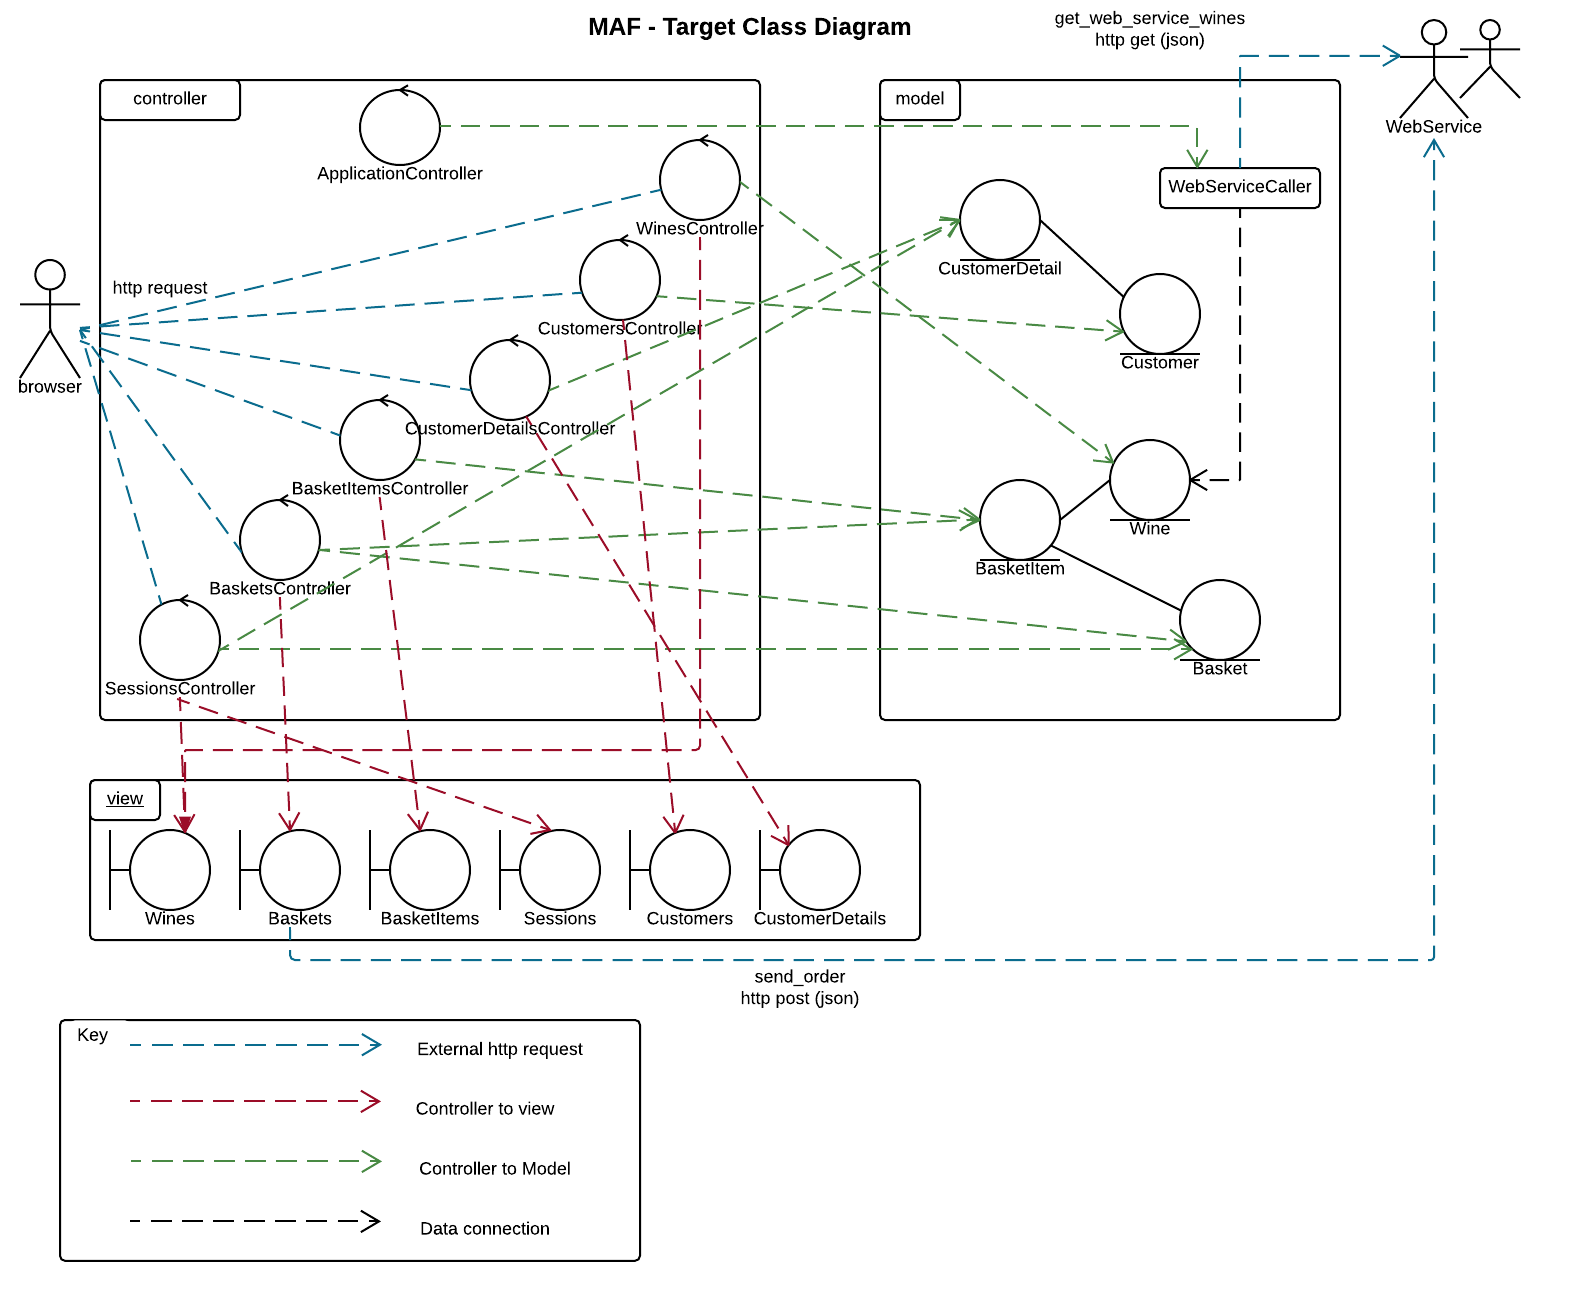
\includegraphics[width=1\textwidth]{assets/MAF_Target_Class_Design}
                \caption{The intended design of the classes and their connections in the MVC pattern.}
                \label{fig: Target Class Diagram.} 
\end{figure}



You can see that the SessionsController interacts with the Basket and CustomerDetail model, in order to keep the customer logged in with a persistent basket while they browse.

To get the Wines, HTTP POST requests are scheduled to be made every 60 seconds to each known Web Service, using rufus-scheduler gem\cite{rufus} and are made asynchronously with SuckerPunch gem\cite{suckerpunch}, from my own class WebServiceCaller. This ensures that a user is not interrupted while they browse and the Wines are always kept up to date without making calls to the Web Suppliers too frequently. 

The WebServiceCaller gets the list of Wines from the Web Services listed in a config file and updates any Wines with different information or that are cheaper than the current known Wine. Wines between different suppliers are distinguished by their product name only, even if their other attributes differ. In a real version of this application, a unique universal identifier would perhaps be more appropriate, such as a bar code.

For the images of the wine bottles, I chose only to get the image url from the Web Service that matches images already in MAF, rather than to link back to the Web Service. Through doing this, the application may be expanded upon later to get an actual copy of the images and store them in assets. I feel this is a better choice than linking back to the original images, as the bandwidth usage would increase on the Supplier web site through our image link back to them.

In order to fulfill the functional requirement of Search, I decided to use Solr with the Sunspot gem \cite{solrsunspot}. This allows for fulltext search and partial text search using NGrams, through any fields set as `searchable' on an entity. The allowing of partial search needs to be set up in the scheme configuration of Solr in order to work, but is very powerful once running. In order to use Solr, we must set up a local Solr server to use, and allow it to reindex our records in order to find them.
\begin{lstlisting}
bundle exec rake sunspot:solr:start # or sunspot:solr:run
rake sunspot:reindex
\end{lstlisting}
There are a number of gems to be used for Search, or even writing a method to do it for us through SQL queries. I chose to use Solr, however, as it had exactly what I needed in order to search through my list of Wines, without me trying to re-implement what it does already.

I chose to keep Customer and CustomerDetails separate, where CustomerDetails actually refers to a customer email and their password digest. By keeping the Customer and CustomerDetails separate, it allows Customers to update their information in the Customer table without affecting or accessing the CustomerDetails. Similarly, if an attacker found their way into the Customer table, they wouldn't have access to the passwords, giving us added security through this separation.

Sending Orders to the Web Service is as simple as when a Customer clicks Checkout (while logged in), the order is sent to a method where a JSON body is built into a POST request for each Wine, and the order(s) is then sent to the respective suppliers of the Wines requested by the order using rest-client\cite{restclient} gem. In a future version of the application, it would be preferable to have Orders kept in the database, to allow a Customer to see their previous orders.

%----------------------------------------------------------------------------------------
%	WEB SERVICE ARCHITECTURE
%----------------------------------------------------------------------------------------

\section{Web Service Architecture}

Since I was new to Rails, I chose to start developing my Web Service first, using Rails over any other language to get comfortable with it. The Web Service only needed to know about two things, Wines and Orders, with RESTful routes to access them, in this case a GET for wines.json, and POST for orders. With this in mind, my target classes before implementation are shown below.

\begin{figure}[H]
        \centering
                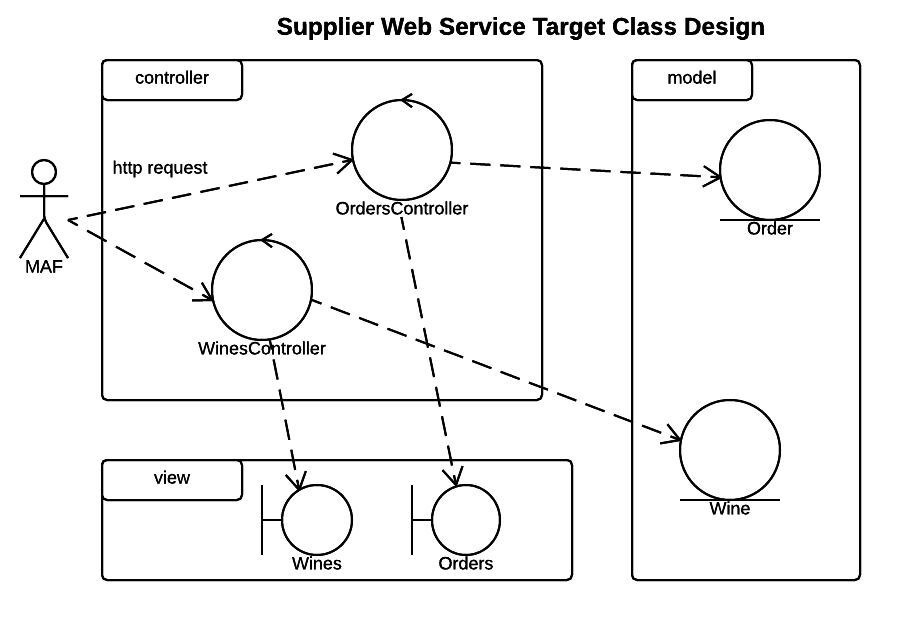
\includegraphics[width=1\textwidth]{assets/Supplier_Web_Service_Target_Class_Design}
                \caption{The intended design of the classes and their connections in the MVC pattern.}
                \label{fig: Target Class Diagram.} 
\end{figure}

Using RESTful endpoints, we don't need to define specific routes for certain things, and can just let Rails handle it as long as we define that Orders and Wines are resources. When providing the Wine data, a GET request comes from MAF to the WinesController that includes a custom HTTP header for when the service was last accessed by the MAF. The Web Service uses the value from this header and gets all Wines in the database that were created or updated after the time MAF last asked for them and returns them in JSON format, e.g.
\begin{lstlisting}
{"id":14,"name":"Abracadabwine","description":"Better than Magic! Tasty!","image_url":"wine6.jpg","price":"5.01","country_of_origin":"Poland","grape_type":"Green","suitable_for_vegetarians":true,"bottle_size":"350ml","url":"http://localhost:3001/wines/14.json","supplier":"Wine Supplier A"}
\end{lstlisting}

Doing this cuts down on the amount of database operations on the MAF side, and the bandwidth used by the Supplier to return the Wines. I originally had a method for deleting Wines no longer existing in any Web Service which worked until I implemented the check to only send wines that had been created or updated since I last called it. The delete function then started deleting all Wines in MAF except those updated. If I were to do this again, I would have a flag on each Wine in the JSON sent by the Web Service that says what status it is in (In Stock, Out of Stock, Discontinued) and use this flag to determine whether to keep or delete a Wine from the MAF database.

When it comes to receiving Orders, the Web Service OrdersController receives a HTTP POST with a body of JSON that it parses into an Order entity and puts into the database if it passes the model validation, which is enough for this prototype. Each order contains the required customer information (name, email, address), the ID of the Wine in the Web Supplier (saved as 'Product Number' in MAF) and the quantity of the Wine to be ordered. I included a view for the Orders so I could see that the Orders were correctly sent by MAF.

%----------------------------------------------------------------------------------------
%	TEST STRATEGY
%----------------------------------------------------------------------------------------

\section{Test Strategy}
\subsection{System Testing}
I focused on implementing the functional requirements through using a system test table, indicating what the system should be like and how it should respond based on assumptions the functional requirements. I wrote my system test table after reading the requirements of the application and gradually went through them one by one as I implemented my design, to ensure my system met the requirements.

The majority of my system tests passed, and completing each functional requirement and fulfilling each system test was pretty satisfying. If this system were more than a prototype, I'd expand on these tests to include more in-depth testing on system validation of user input, the security of sessions and more examples of searching for Wines using Solr. The system test table and my results can be seen below.

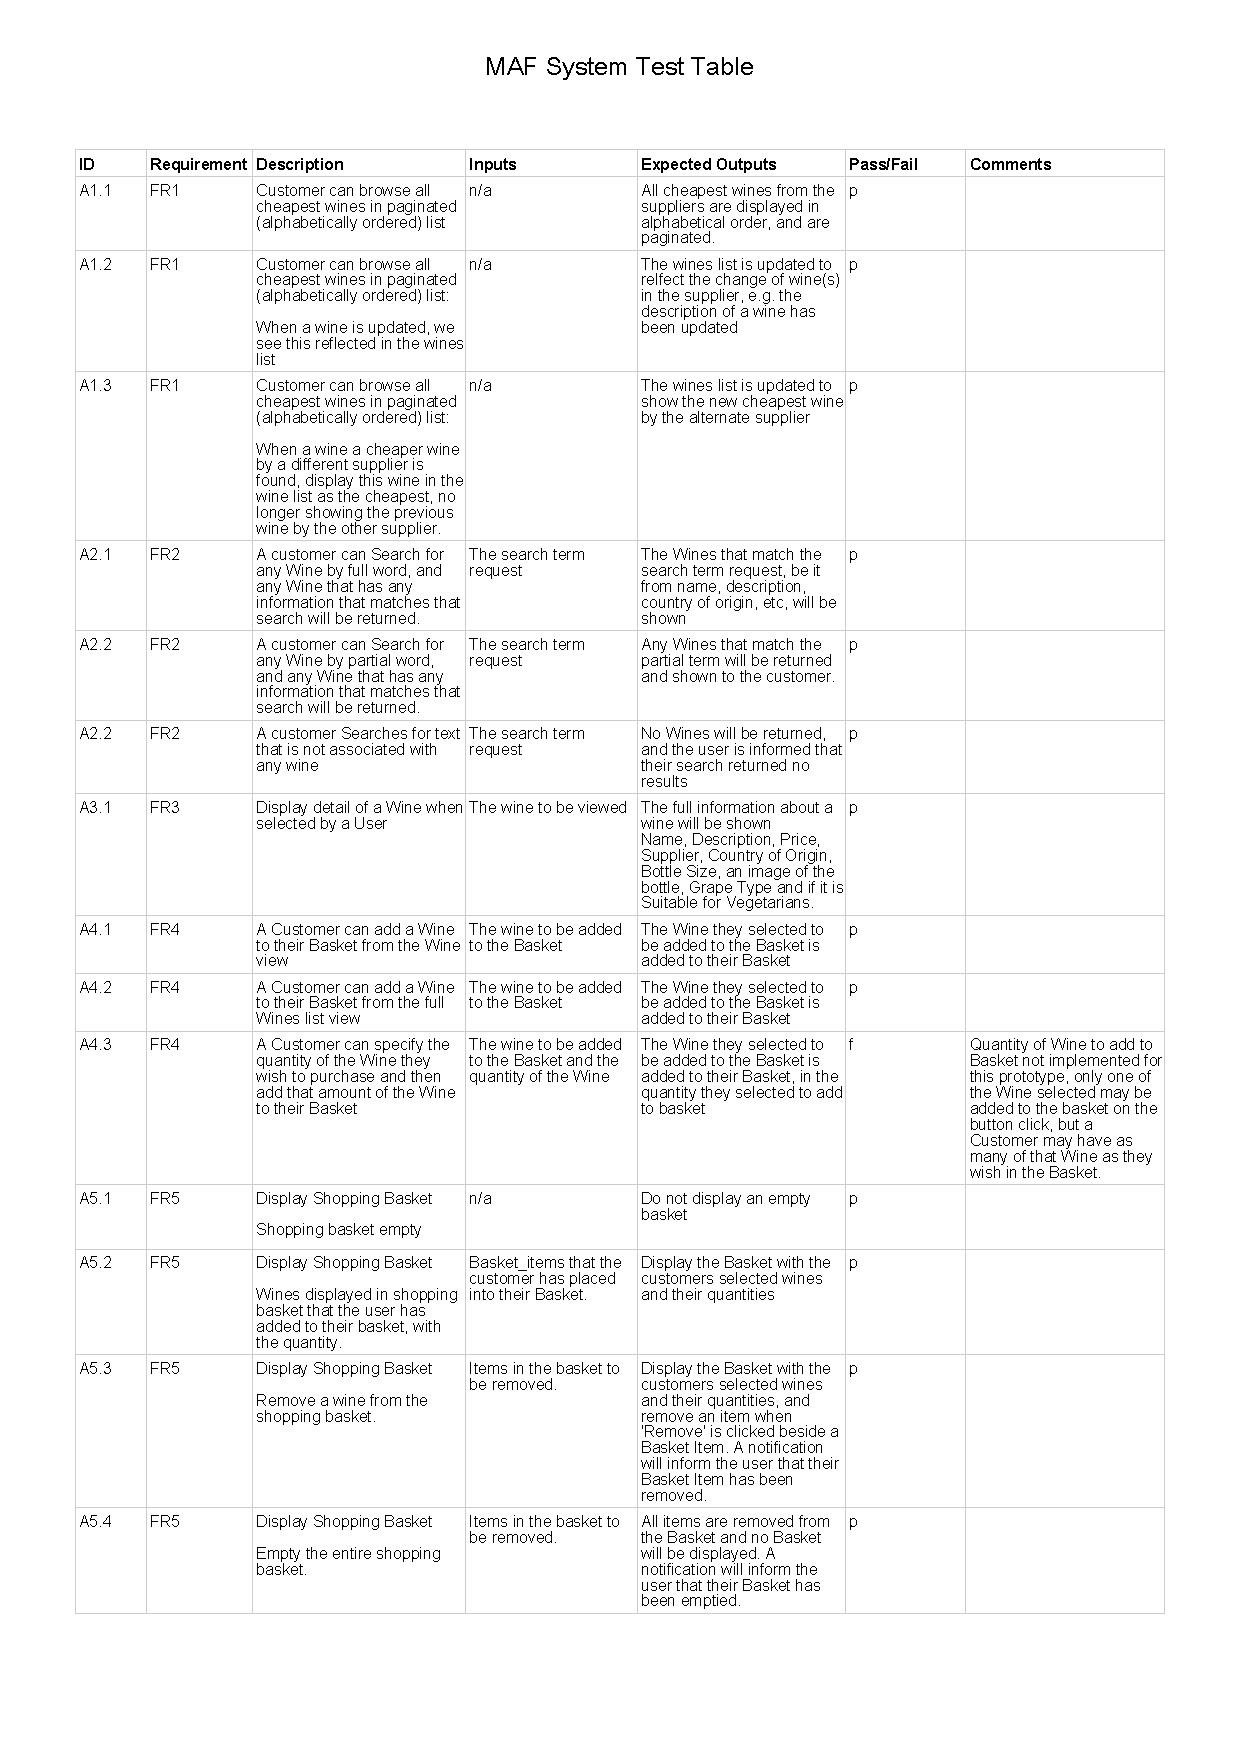
\includepdf[pages=-]{assets/MAF_System_Test_Table.pdf}

In order to back up my system test table, along with the screen cast provided with the application and this report, I have included some screenshots of the application in various stages of the system tests. Not all tests have been included in the screenshots, and some tests are difficult to give examples for through screenshots alone.

\begin{figure}[H]
        \centering
                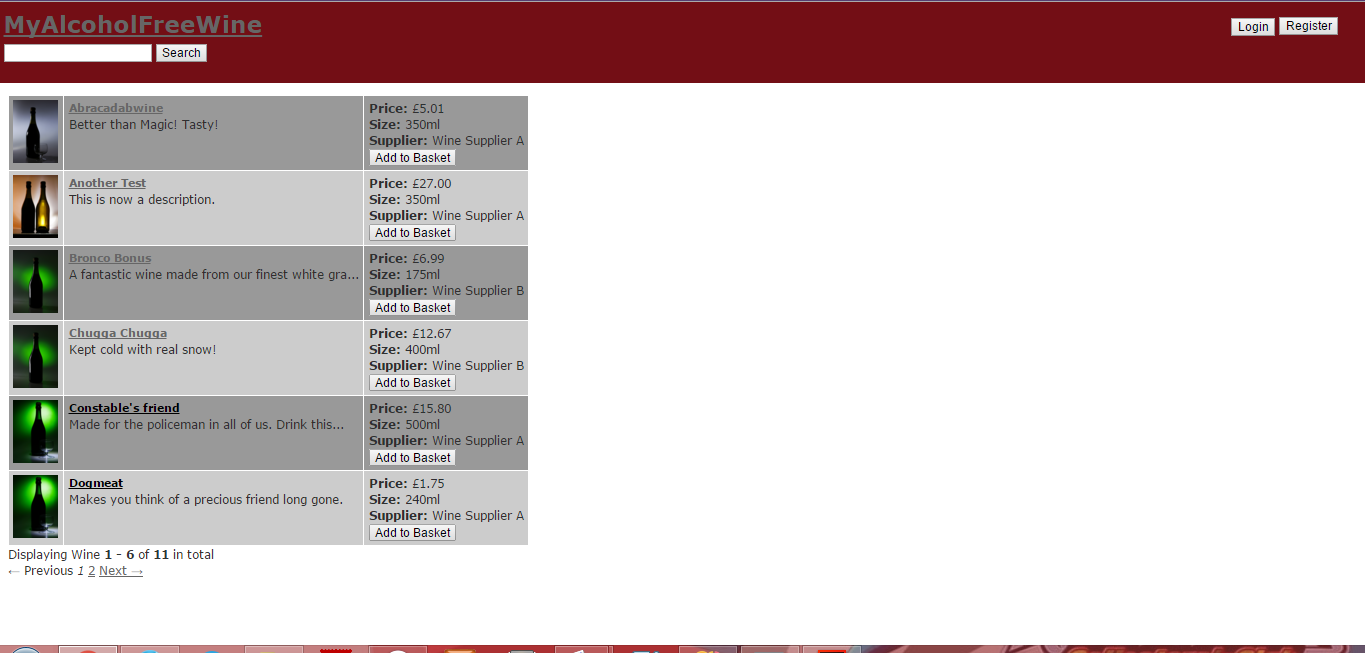
\includegraphics[width=1\textwidth]{assets/FR1_screen_1}
                \caption{FR1 - Displaying a list of cheapest Wines.}
                \label{fig: FR1_1.} 
\end{figure}
The system presents the user with a number of Wines, provided by the Web Services. If a Wine in a Web Service updates, we can see the change reflected here. Through testing this requirement I was able to see when the bug of all wines except those recently updated were deleted appeared and fix it.

\begin{figure}[H]
    \centering
    \begin{subfigure}[b]{0.3\textwidth}
        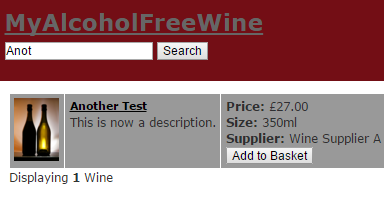
\includegraphics[width=\textwidth]{assets/FR2_screen_1}
        \caption{Search using partial text to find a Wine}
        \label{fig:FR2 partial}
    \end{subfigure}
    ~ %add desired spacing between images, e. g. ~, \quad, \qquad, \hfill etc. 
      %(or a blank line to force the subfigure onto a new line)
    \begin{subfigure}[b]{0.3\textwidth}
        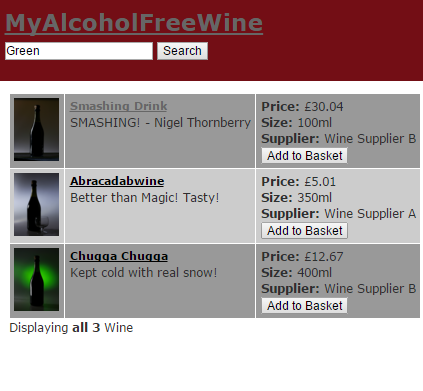
\includegraphics[width=\textwidth]{assets/FR2_screen_2}
        \caption{Searching Green for Grape Type}
        \label{fig:FR2 full search}
    \end{subfigure}
    ~ %add desired spacing between images, e. g. ~, \quad, \qquad, \hfill etc. 
    %(or a blank line to force the subfigure onto a new line)
    \begin{subfigure}[b]{0.3\textwidth}
        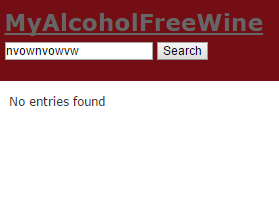
\includegraphics[width=\textwidth]{assets/FR2_screen_3}
        \caption{Searching something that won't give results}
        \label{fig:FR2 nonsense}
    \end{subfigure}
    \caption{FR2: Using the Search bar}\label{fig:FR2 Search}
\end{figure}

\begin{figure}[H]
        \centering
                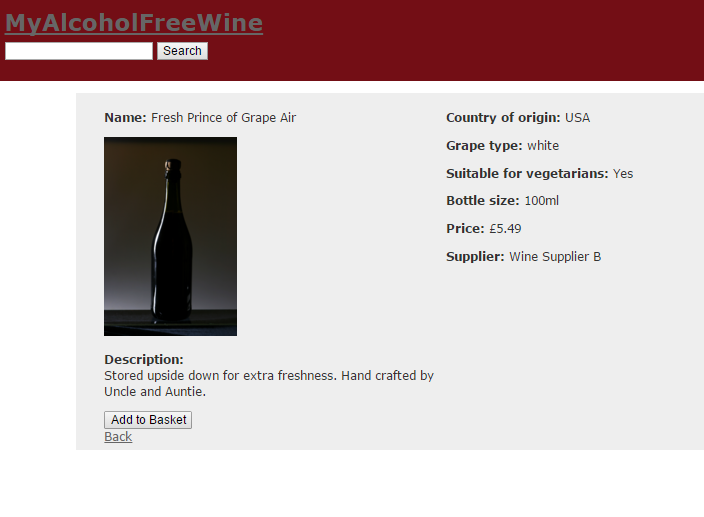
\includegraphics[width=0.7\textwidth]{assets/FR3_screen}
                \caption{FR3 - Displaying the full info for a Wine, FR4 allowing the Wine to be added to the Basket.}
                \label{fig: FR3_1.} 
\end{figure}

\begin{figure}[H]
    \centering
    \begin{subfigure}[b]{0.4\textwidth}
        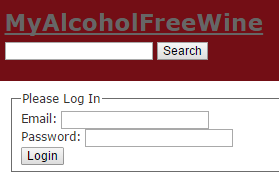
\includegraphics[width=\textwidth]{assets/FR7_screen_1}
        \caption{The login form}
        \label{fig:FR7 Login}
    \end{subfigure}
    ~ %add desired spacing between images, e. g. ~, \quad, \qquad, \hfill etc. 
      %(or a blank line to force the subfigure onto a new line)
    \begin{subfigure}[b]{0.4\textwidth}
        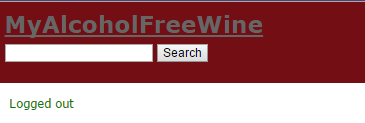
\includegraphics[width=\textwidth]{assets/FR7_screen_2}
        \caption{Informing the Customer that they have Logged out}
        \label{fig:FR7 Logout}
    \end{subfigure}
    \caption{FR7: Customer account actions}\label{fig:FR7 Customer Account 1}
\end{figure}

\begin{figure}[H]
    \centering
    \begin{subfigure}[b]{0.4\textwidth}
        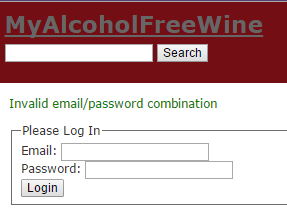
\includegraphics[width=\textwidth]{assets/FR7_screen_3}
        \caption{With invalid email/password}
        \label{fig:FR7 Bad data}
    \end{subfigure}
    ~ %add desired spacing between images, e. g. ~, \quad, \qquad, \hfill etc. 
    %(or a blank line to force the subfigure onto a new line)
    \begin{subfigure}[b]{0.4\textwidth}
        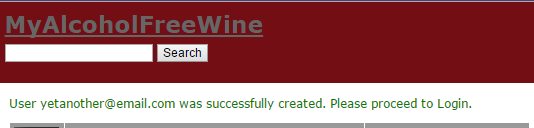
\includegraphics[width=\textwidth]{assets/FR7_screen_6}
        \caption{Successfully creating a customer account}
        \label{fig:FR7 Duplicate email}
    \end{subfigure}
    \caption{FR7: Customer account actions}\label{fig:FR7 Customer Account 2}
\end{figure}

There are a number more system tests that could be done, and if this were a full project I would have system tests for every route that could be accessed, add security to the customer sessions, potentially use Selenium for automating tests of browsing the web site as a user to see what happened under certain conditions and more. As the majority of the conditions laid out in my functional requirements systems test table pass, I am pleased with these results. However, if given more time I would like to look into other ways of testing the system to be sure that it was as foolproof as possible.

\subsection{Unit Test for models and controllers}
For testing the innards of my application, I used Rails unit testing for my models and controllers. Some of the generated tests by Rails were no longer required, as I didn't need actions for things such as New for Wines, as they are added into the database by the WebServiceCaller and not required to be added manually in MAF.

The majority of my Controller unit tests are ensuring that new objects are created when requesting, and importantly that the user is redirected to where they need to go. An example is when a User creates a basket item (adding an item to a Basket). I don't want a user to go to the Basket items list and see a bunch of items from all Baskets, and so they are instead redirected to their particular Basket\_path.

My unit tests for the models are mainly checking the validation, that no entities will be created that violate the conditions of their existence or creation. This ensures things a Customer always having an email address, and that it is unique to itself. 

\begin{figure}[H]
        \centering
                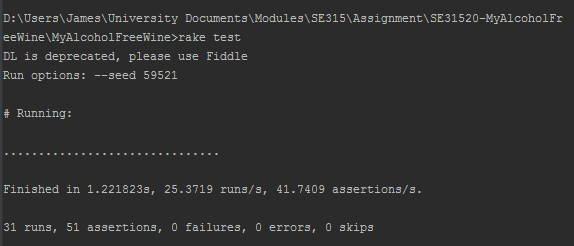
\includegraphics[width=1\textwidth]{assets/unit_test}
                \caption{Asking rake to run all test for my MAF project.}
                \label{fig: running tests.} 
\end{figure}

%----------------------------------------------------------------------------------------
%	SELF-EVALUATION
%----------------------------------------------------------------------------------------

\section{Self-Evaluation}

\subsection{Summary}
Overall, I'm relatively happy with the result of this assignment. While I don't have full confidence that everything I have done and my design decisions are correct, I feel like I've learned a large amount. Before the assignment I wasn't comfortable writing in Ruby on Rails, and not too sure on routing. Now I feel happy enough that I could attempt to write more Rails apps and have enough experience to get going by myself.

I know there are areas for improvement (security, persistent sessions and baskets, better tests, etc), but as far as the time allowed, my understanding and learning of Rails and this assignment tasking me to just create a prototype, I am happy with the resulting program. I appreciated the help and starting point of the Agile Web Development with Rails\cite{railsbook} book, and think if I were to re-implement this application with better knowledge, I would still use many ideas from this book to begin with and build upon them just as I have done for this.

During implementation, I found the most difficult part to be implementing routing, and getting my links in the views to execute the correct controller actions as I wanted (for the more complex tasks, such as removing the last item from a basket, logging in and sending the webservice order). Doing this assignment helped me get my head around routing. With little knowledge of Rails, it was difficult to get started, but once I got into the flow of development and started to understand more how Ruby on Rails works, it became much easier and more enjoyable. 

\subsection{Mark Breakdown}
\subsubsection{Screen cast}
My screen cast shows my MAF fulfilling the functional requirements set out by the assignment, and two Web Services running with separate data and MAF communicating with them.
\newline
Mark: 9/10\%

\subsubsection{Design}
My sections for the architecture of MAF and the Web Service both display diagrams for my classes (MVC) and there is a diagram to show the relationships between my tables in the database for MAF. I have described the way in which my application works and why I chose certain ways of implementation. My Rails knowledge is not fantastic, but I did the best I could with what I know to design a system in the `Rails way' and use MVC appropriately to design a system that would fulfill the requirements.
\newline
Mark: 17/20\%

\subsubsection{Implementation: MAF}
My MAF application runs, using Rails the architecture for MVC and communicates with the Web Services. The code is commented where appropriate, identifier names make sense for what they represent and adheres to DRY. Data manipulation is handled in the Models, Views stay away from logic code and Controllers are thin, getting data from model methods and enabling the views to display it as necessary.
\newline
Mark: 23/25\%

\subsubsection{Implementation: Web Service}
One Web Service application was built, with two instances of it able to be run, with different data sets. The resources for the Web Service are RESTful and requested are correctly routed to GET and POST requests where appropriate (wines, orders). The Web Service only returns those items that have been updated since the MAF last called to improve efficiency of sending data.
\newline
Mark: 15/15\%

\subsubsection{Testing}
There are unit tests for each controller, and more than just the ones generated by rails, and unit tests for the models where appropriate for the validations and logic methods. There is a system test table that matches my assumed customer expectations. I have discussed the results and how I used the system test table to work through the functional requirements. There are, however, no cucumber tests and testing could cover more areas.
\newline
Mark: 10/15\%

\subsubsection{Evaluation}
I have indicated the results I believe I would receive for each section defined by the marking grid and why. I have a summary of my evaluation to discuss what I found challenging or easy about the assignment, and what I learned through doing it.
\newline
Mark: 5/5\%

\subsubsection{Flair}
I have demonstrated some flair through my implementation of Search using Solr with Sunspo, calling the WebService asynchronously with scheduling and only retrieving the latest updates to wines to cut costs on database operations. If I had more time I would try deployment to Heroku, better CSS design with Bootstrap and more user controls.
\newline
Mark: 5/10\%

\subsubsection{Total}
Mark: 84/100\%



%----------------------------------------------------------------------------------------
\clearpage

%----------------------------------------------------------------------------------------
%	REFERENCES
%----------------------------------------------------------------------------------------

\begin{thebibliography}{5}

\bibitem{assignment} Chris Loftus, ``MyAlcoholFreeWine.com'',SE31520/CHM5820 Assignment 2015-16, October 27 2015

\bibitem{stockvault} Stockvault.net, 'Stockvault.net - Free wine Stock Photos', 2015. [Online]. Available: http://www.stockvault.net/search/?query=wine. [Accessed: 06- Dec- 2015].

\bibitem{railsbook} D. Thomas, D. Hansson and L. Breedt, Agile web development with rails. Raleigh, N.C.: Pragmatic Bookshelf, 2005.

\bibitem{rufus} GitHub, 'jmettraux/rufus-scheduler', 2015. [Online]. Available: https://github.com/jmettraux/rufus-scheduler. [Accessed: 06- Dec- 2015].

\bibitem{suckerpunch} GitHub, 'brandonhilkert/sucker\_punch', 2015. [Online]. Available: https://github.com/brandonhilkert/sucker\_punch. [Accessed: 06- Dec- 2015].

\bibitem{solrsunspot}  Sunspot.github.io, 'Sunspot: Solr-powered search for Ruby objects', 2015. [Online]. Available: http://sunspot.github.io/. [Accessed: 06- Dec- 2015].

\bibitem{restclient} GitHub, 'rest-client/rest-client', 2015. [Online]. Available: https://github.com/rest-client/rest-client. [Accessed: 07- Dec- 2015].

\end{thebibliography}


\end{document}


